\newpage
\section{Анализ предметной области}
\label{sec:Background}
\subsection{Описание предметной области}
\label{subsec:Description}

Сайты для хостинга открытого исходного кода, такие как GitHub, например, GitLab, Bitbucket и др, представляют собой цифровые площадки, где разработчики могут хранить, управлять и совместно работать над своими проектами с открытым доступом к исходному коду.

Одной из основных причин популярности таких платформ является идеология открытого исходного кода. Распространение проектов с открытым исходным кодом способствует коллективному развитию программного обеспечения, позволяя разработчикам из разных уголков мира вносить свой вклад, исправлять ошибки и улучшать функционал. Это приводит к созданию более качественного, надежного и инновационного программного обеспечения.

Сами сайты основаны на системах контроля версий, которые являются ключевым инструментом в разработке программного обеспечения, обеспечивая эффективное управление изменениями в исходном коде проекта. Они позволяют разработчикам отслеживать и сохранять историю изменений в коде, а также управлять конфликтами и совмещать работу множества разработчиков. Согласно рейтингу Tagline~\cite{SCVRating} самой популярной системой контроля версий считается Git, что представлено на рисунке~\ref{ris:scvrating}.

\begin{figure}[h]
    \centering
    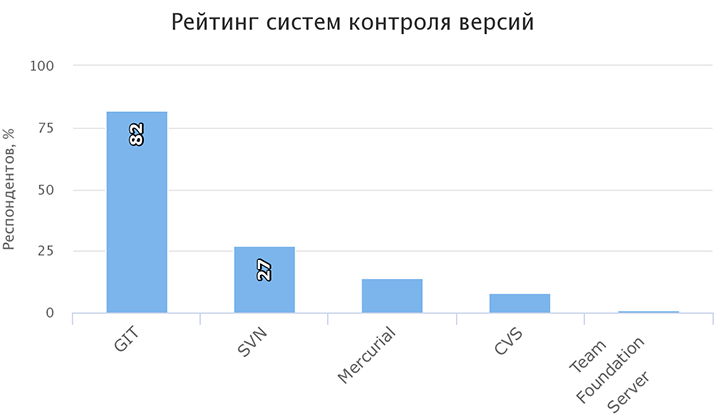
\includegraphics[width=0.9\linewidth]{pic/scvrating.png}
    \vspace{1em}
    \caption{Рейтинг систем контроля версий}
    \label{ris:scvrating}
\end{figure}
\vspace{1em}

Git, созданный Линусом Торвальдсом в 2005 году, стал стандартом для управления исходным кодом в различных проектах, от небольших локальных до масштабных проектов с открытым исходным кодом, таких как ядро Linux и сам GitHub.

GitHub -- это веб-платформа для хранения и совместной разработки проектов с открытым исходным кодом. С момента своего запуска в 2008 году GitHub стал одной из самых популярных и важных платформ для разработчиков по всему миру. Его привлекательность обусловлена множеством факторов. Так, издание The New Stack~\cite{GitRating} собрало статистику по используемым хостингам кода на основе Git за 2018-2019 года (рис.~\ref{ris:gitrating}). Несмотря на падение популярности GitHub в 2019 году по сравнению с 2018, он все еще остается самым используемым сайтом для расположения своего кода в рамках репозиториев.

\begin{figure}[h]
    \centering
    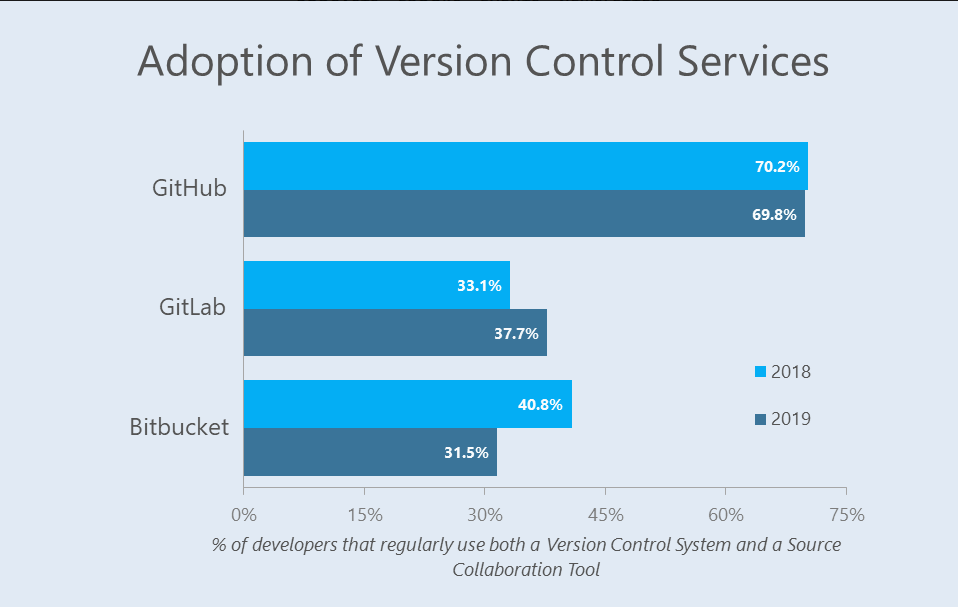
\includegraphics[width=1\linewidth]{pic/gitrating.png}
    \vspace{-1em}\caption{Рейтинг хостингов кода на основе Git}
    \label{ris:gitrating}
\end{figure}
\vspace{1em}

Каждый проект на GitHub представлен в виде репозитория, где хранятся файлы проекта и история их изменений. Для отслеживания действий других пользователей с текущим репозиторием на GitHub используются различные параметры.

\begin{enumerateparendot}
    \item Звезды (Stars): Звезды представляют собой показатель популярности проекта. Пользователи GitHub могут добавлять звезды к проектам, которые им нравятся или которые они хотят отслеживать. Чем больше звезд у проекта, тем он популярнее.

    \item Форки (Forks): Форки представляют собой копии репозитория проекта, созданные другими пользователями. Форк может использоваться для внесения изменений в проект без изменения оригинального кода. Чем больше форков у проекта, тем больше разработчиков заинтересовано в его доработке и участии.

    \item Проблемы (Issues): Проблемы представляют собой список задач, багов или идей для улучшения проекта. Количество проблем может служить показателем активности и вовлеченности сообщества в развитие проекта.

    \item Запросы на слияние (Pull Requests): Запросы на слияние представляют собой предложения от разработчиков о внесении изменений в код проекта. Они могут быть использованы для исправления ошибок, добавления нового функционала или внесения других улучшений.
\end{enumerateparendot}

Все эти метрики помогают разработчикам оценивать популярность и активность проектов на GitHub. Звезды и форки позволяют судить о популярности проекта среди пользователей, а проблемы и запросы на слияние -- об активности и вовлеченности сообщества разработчиков.

Использование GitHub и его метрик стало стандартной практикой в сообществе разработчиков благодаря его открытости, удобству использования и широким возможностям для совместной работы и обмена знаниями.
\vspace{1em}

\subsection{Обзор аналогов и существующих решений}
\label{subsec:Analogues}

Исследования, посвященные анализу данных, связанных с использованием платформы GitHub и разработкой программного обеспечения на этой платформе, являются актуальной и распространенной темой для научных исследований.

Так, авторы статьи~\cite{abs-2308-14211} обсуждают проблему классификации отзывов о приложениях, которые содержат важную информацию о потребностях пользователей. Исследователи предлагают подход для создания более обобщенной модели, используя информацию из системы отслеживания задач GitHub, которая содержит ценные данные о потребностях пользователей. После проведения экспериментов, они показывают, что использование размеченных задач из GitHub может улучшить точность и полноту классификации отзывов, особенно для отчетов о багах и запросов на новые функции. 

В работе~\cite{RoccoRSNR23} поднимается важность репозиториев программного обеспечения для управления проектами, включая исходный код, документацию и отчеты об ошибках. Особое внимание уделяется платформе GitHub, которая для помощи разработчикам в поиске подходящих артефактов использует темы (topics), являющимися короткими текстами, присваиваемыми хранимым артефактам. Однако неправильное присвоение тем может негативно сказаться на популярности репозитория. 

Закария Альшара и другие авторы в своей статье~\cite{AlsharaSSS23} рассматривают проблему управления задачами (issues) на платформе GitHub, особенно в случае быстрого роста числа создаваемых задач. Для помощи разработчикам в обработке задач существуют внешние участники, которые исправляют задачи, создавая pull-запросы (Pull Requests, они же PR). Однако часто такие PR не связываются с соответствующими задачами (issues), что затрудняет управление проектом. В статье предлагается использование моделей машинного обучения (ML) для автоматического восстановления связей между PR и задачами на GitHub. Установление связей между PR и задачами ценно, так как это помогает улучшить управление разработкой и обслуживанием проектов, что влияет на популярность и развитие проекта в дальнейшем.

В работе~\cite{RamasamySBB23} исследует, как проводится кодирование в области науки о данных на GitHub. Авторы анализируют, как данные ученые переходят между разными этапами работы с данными. Результаты исследования показывают, что кодирование имеет определенные паттерны. Кроме того, авторы попытались обучить модели машинного обучения для предсказания этапов работы с данными и достигли точности примерно 71\%.

О популярных проектах говорят в статье Джесси Айала и ее коллеги~\cite{AyalaG23}, а именно о важности использования непрерывной интеграции и поставки и политики безопасности в известных и пользующихся интересом проектах с открытым исходным кодом, особенно на GitHub. Исследование показало, что многие проекты не активно используют эти возможности, и призывает управляющих таких проектов уделить им больше внимания для предотвращения уязвимостей. 

Кроме того, в исследовании~\cite{PuhlfurssMM22} фокусируются на том, как документируется информация о функциональных возможностях программного обеспечения в проектах на GitHub и связана ли она с исходным кодом. Авторы провели анализ 25 популярных репозиториев на GitHub и обнаружили, что хотя документация о функциональности часто присутствует в различных текстовых файлах, она часто неструктурированна, и связь с исходным кодом редко устанавливается, что может привести к затруднениям в его поддержке на долгосрочной перспективе. 

Статья~\cite{CasalnuovoSRR17} рассматривает инструмент GitcProc, который предназначен для анализа проектов на GitHub. Этот инструмент позволяет извлекать информацию о разработке, включая исходный код и историю исправления ошибок. GitcProc может отслеживать изменения в исходном коде и связывать их с функциями с минимальными настройками. Он успешно работает с проектами на разных языках программирования, обнаруживая исправления ошибок и контекст изменений в коде. 

Помимо этого, стоит также рассмотреть работу~\cite{SollV17}, где авторы обсуждают задачу классификации репозиториев на GitHub, которая представляет собой сложную задачу. Они представляют алгоритм ClassifyHub, основанный на методах ансамблирования, разработанный для соревнования InformatiCup 2017. Этот алгоритм успешно решает задачу классификации с высокой точностью и полнотой, что может быть полезно для различных приложений, таких как рекомендательные системы.

Самой приближенной к поставленной задаче статьей является <<A Cross-Repository Model for Predicting Popularity in GitHub>>~\cite{abs-1902-05216}, в которой рассматривается создание модели для прогнозирования популярности репозиториев на GitHub, используя данные из разных репозиториев. Модель, основанная на рекуррентной нейронной сети LSTM, позволяет более точно предсказывать популярность, чем стандартные методы прогнозирования временных рядов на основе данных из одного репозитория. 

Кроме нее, есть также исследование~\cite{HanDXWY19}, в котором предлагают метод для прогнозирования популярности проектов на GitHub. Он использует 35 признаков, извлеченных из GitHub и Stack Overflow, чтобы классифицировать проекты как популярные или нет. Основными признаками для определения популярности оказались количество веток, количество открытых задач и количество участников проекта.
\vspace{1em}

\subsection{Теоретический базис}
\label{sec:Models}

В этом разделе рассматриваются основные концепции и методы машинного обучения, которые лежат в основе разработки моделей для классификации и регрессии. Машинное обучение -- это раздел искусственного интеллекта, который изучает методы анализа данных и построения предсказательных моделей без явного программирования. Одним из ключевых направлений в машинном обучении является обучение с учителем, где модели создаются на основе предварительно размеченных данных~\cite{books_daglib_0033642}. Чаще встречаются модели двух типов: модель классификации и модель регрессии.

\textit{Модели классификации} являются методами обучения с учителем, цель которых заключается в том, чтобы прогнозировать принадлежность объекта к одной из заданных категорий или классов на основе набора предварительно размеченных данных. Модели классификации используют алгоритмы, которые находят закономерности в данных и создают функцию, относящую новый объект к одному из заранее определенных классов.

Рассмотрим модели, которые будут использованы для работы.
\vspace{1em}

\subsubsection*{Decision Tree (Дерево решений)}
    
Дерево решений строит структуру в виде дерева, в которой каждый узел представляет собой тест на значение определенного признака, а каждое ребро - результат этого теста~\cite{izza2020explaining}. Для построения дерева используются различные алгоритмы. Процесс построения дерева продолжается, пока не будет выполнен какой-то критерий останова, например, достигнута максимальная глубина дерева или узел содержит объекты только одного класса. Алгоритм построения дерева решений представлен в виде диаграммы деятельности на рисунке~\ref{ris:activity}.

\begin{figure}[H]
    \centering
    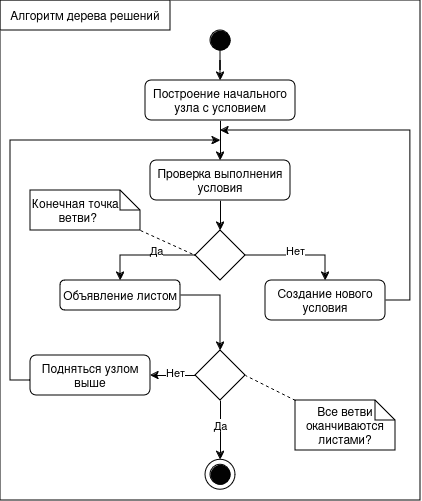
\includegraphics[width=0.9\linewidth]{pic/activity.png}
    \vspace{1em}\caption{Алгоритм дерева решений}
    \label{ris:activity}
\end{figure}
\vspace{1em}

\subsubsection*{Random Forest (Случайный лес)}

Random Forest строит ансамбль деревьев решений, каждое из которых обучается на случайной подвыборке данных~\cite{breiman2001random}. В процессе построения дерева для каждого разбиения выбирается случайный поднабор признаков. После построения всех деревьев в ансамбле, предсказание производится путем агрегации результатов всех деревьев, например, путем голосования (в случае классификации) или усреднения (в случае регрессии).
\vspace{1em}

\subsubsection*{Gradient Boosting (Градиентный бустинг)} 

Gradient Boosting последовательно обучает слабые модели, каждая из которых предсказывает остатки (разницу между истинными значениями и предсказанными значениями) предыдущей модели~\cite{hastie2001elements}. На каждом шаге минимизируется функция потерь (например, среднеквадратичная ошибка для задачи регрессии) с помощью градиентного спуска. Таким образом, каждая новая модель исправляет ошибки предыдущей модели.
\vspace{1em}

\subsubsection*{AdaBoost}
    
AdaBoost обучает слабые модели на последовательно изменяющихся весах обучающих образцов~\cite{Hastie2009MulticlassA}. На каждой итерации модель фокусируется на объектах, которые были классифицированы неправильно на предыдущих итерациях. После обучения всех моделей, их прогнозы комбинируются с помощью взвешенного голосования.
\vspace{1em}

\subsubsection*{Gaussian Naive Bayes (Наивный байесовский классификатор)}

Этот классификатор основан на применении теоремы Байеса с допущением о независимости между признаками~\cite{Zhang2004}. Он предполагает, что каждый признак влияет на класс независимо от других признаков. При классификации модель оценивает вероятность принадлежности объекта к каждому классу и выбирает класс с наибольшей вероятностью.
\vspace{1.5em}

\textit{Модели регрессии} также являются методами обучения с учителем, но в отличие от классификации, их цель состоит в прогнозировании непрерывных значений целевой переменной на основе имеющихся данных. Модели регрессии стремятся к поиску математической функции, которая наилучшим образом описывает связь между входными признаками и выходными значениями.
\vspace{1em}

\subsubsection*{Linear Regression (Линейная регрессия) }

Линейная регрессия моделирует линейную зависимость между предикторами и целевой переменной. Она находит коэффициенты линейной функции таким образом, чтобы минимизировать сумму квадратов разностей между наблюдаемыми и предсказанными значениями.

Для моделей регрессии Decision Tree, Random Forest, Gradient Boosting главное отличие от их использования в классификации заключается в том, как они строят свои прогнозы и как оценивают качество модели~\cite{Nunez2011}. Так, Случайный лес после обучения всех деревьев результаты агрегируются, например, путем усреднения, чтобы получить окончательный прогноз, а для регрессионных Деревьев решений обычно используется критерий ветвления, такой как среднеквадратичная ошибка.
